\documentclass[conference]{IEEEtran}
\IEEEoverridecommandlockouts
% Based on the official IEEE conference template (conference_101719.tex, IEEEtran).
\usepackage{cite}
\usepackage{amsmath,amssymb,amsfonts}
\usepackage{graphicx}
\usepackage{textcomp}
\usepackage{xcolor}
\usepackage{booktabs}
\usepackage{multirow}
\usepackage{tikz}
\usepackage{pgfplots}
\pgfplotsset{compat=1.18}
\usetikzlibrary{positioning,arrows.meta,fit}


% Starts a new row of authors, so four authors sit as 2 + 2.
\makeatletter
\newcommand{\linebreakand}{\end{@IEEEauthorhalign}\hfill\mbox{}\par\mbox{}\hfill\begin{@IEEEauthorhalign}}
\makeatother

\begin{document}

\title{Multimodal News Summarization with Relevance-Filtered Heterogeneous Sources\thanks{An AI assistant (Claude, Anthropic) was used to draft the text of this paper. The authors reviewed the text and results and take responsibility for them.}}

\author{
\IEEEauthorblockN{1\textsuperscript{st} S Samraj Pishey}
\IEEEauthorblockA{\textit{SoCSE} \\
\textit{RV University}\\
Bengaluru, India \\
ssamrajpisheybtech24@rvu.edu.in}
\and
\IEEEauthorblockN{2\textsuperscript{nd} S A Shashwath}
\IEEEauthorblockA{\textit{SoCSE} \\
\textit{RV University}\\
Bengaluru, India \\
sashashwathbtech24@rvu.edu.in}
\linebreakand
\IEEEauthorblockN{3\textsuperscript{rd} Rohan Olekar S G}
\IEEEauthorblockA{\textit{SoCSE} \\
\textit{RV University}\\
Bengaluru, India \\
rohanolekarbtech24@rvu.edu.in}
\and
\IEEEauthorblockN{4\textsuperscript{th} Ranjith Kumar P S}
\IEEEauthorblockA{\textit{SoCSE} \\
\textit{RV University}\\
Bengaluru, India \\
ranjithkumarpsbtech24@rvu.edu.in}
}

\maketitle

% ===========================================================================
\begin{abstract}
News stories are now published as a bundle of text, photographs, captions and video, yet most automatic summarizers read only the article. This paper presents a low-cost framework that converts other modalities to text, filters them for relevance, and passes them to a fine-tuned BART summarizer. We evaluate it on a leakage-controlled split of the MM-AVS dataset. Fine-tuning raises ROUGE-1 from 39.99 to 42.48. Adding all image captions gains a further 1.45 ROUGE-1 and 2.12 ROUGE-2 points. Where selections differ, captions chosen with CLIP beat randomly chosen captions by 1.7--1.9 points. Whisper transcripts help only after filtering: relevant transcripts add 1.98 ROUGE-1 points on the stories that receive them, whereas unfiltered transcripts lower ROUGE-L by 0.68. In a human study, CLIP selected the preferred cover image 40.2\% of the time, against 27.7\% for the first image. We also find that 14.5\% of Daily Mail test stories have a reference highlight that nearly copies a caption, and most of the caption gain falls in those stories, so ROUGE gains on this dataset must be read with care.
\end{abstract}

\begin{IEEEkeywords}
multimodal summarization, abstractive summarization, BART, CLIP, Whisper, MM-AVS
\end{IEEEkeywords}

% ===========================================================================
\section{Introduction}
Online news rarely consists of text alone. A typical story combines an article with photographs, captions and an embedded video, and each of these sources can carry information about what matters in the story. A summarizer that draws on such heterogeneous sources has to decide which of them to use and how to combine them. We study multimodal news summarization on MM-AVS~\cite{fu2021mmavs}, a public dataset that packages all of these modalities for CNN and Daily Mail stories.

Pretrained text models such as BART~\cite{lewis2020bart}, PEGASUS~\cite{zhang2020pegasus} and T5~\cite{raffel2020t5} perform well on news but see only the article. Multimodal models usually fuse visual features inside the encoder~\cite{yu2021vgbart,liang2023sov}, which adds parameters and training cost. There is also a less discussed problem: the extra material is not always about the story. In our data, only about half of the speech transcripts are measurably related to their article, and many videos are generic clips. Adding a modality without checking it can therefore add noise.

We keep the summarizer text-only and convert each modality to text. A pretrained model or a similarity measure then decides which pieces are relevant: CLIP~\cite{radford2021clip} for images and TF-IDF similarity for Whisper~\cite{radford2023whisper} transcripts. The whole pipeline runs on one free cloud GPU and an 8\,GB laptop. Our contributions are:
\begin{itemize}
\item a leakage-controlled MM-AVS split with near-duplicate grouping and repaired reference summaries;
\item a controlled comparison of caption selection, using random selection as a control;
\item a relevance filter for speech transcripts, showing that unfiltered speech does not help while filtered speech does;
\item an analysis of where the measured gain comes from, together with a human study of cover-image selection.
\end{itemize}

% ===========================================================================
\section{Related Work}
\textit{Text summarization.} BART~\cite{lewis2020bart}, PEGASUS~\cite{zhang2020pegasus} and T5~\cite{raffel2020t5} established pretraining as the standard route to abstractive summarization, and BRIO~\cite{liu2022brio} improved results by training on the ranking of candidate summaries. Two weaknesses remain relevant here. Abstractive models can introduce content that is not supported by the source~\cite{maynez2020faithfulness,kryscinski2020factcc}, and ROUGE captures quality only in part~\cite{fabbri2021summeval}.

\textit{Multimodal summarization.} Jangra et al.~\cite{jangra2023survey} survey the field. For video with transcripts, Liu et al.~\cite{liu2020multistage} proposed multistage fusion with a forget gate, and Yu et al.~\cite{yu2021vgbart} added attention-based visual layers to BART and T5. For images with text, UniMS~\cite{zhang2022unims} builds on BART and uses knowledge distillation to select an output image, while Liang et al.~\cite{liang2023sov} add auxiliary tasks to make visual features more useful for summarization. SITA~\cite{jiang2023sita} is the closest to our caption stage: it aligns each image with an article sentence and treats that sentence as a pseudo caption. We instead use the captions published with the story. Relevant datasets include MM-AVS~\cite{fu2021mmavs}, whose authors report that external information assists summarization, and MMSum~\cite{qiu2024mmsum} for video.

\textit{Pretrained models as tools.} CLIP~\cite{radford2021clip} scores image--text similarity without task-specific training, BLIP~\cite{li2022blip} generates captions, and Whisper~\cite{radford2023whisper} transcribes noisy web audio. We use such models frozen, as selectors and converters rather than as fused encoders. Our work differs from the studies above in three ways: modalities reach the summarizer only as text, relevance filtering is explicit, and each selection method is compared with a random or unfiltered control at small compute cost. Table~\ref{tab:related} summarizes these differences.

\begin{table}[t]
\caption{Multimodal summarization work compared with this paper.}
\label{tab:related}
\centering
\footnotesize
\setlength{\tabcolsep}{3pt}
\begin{tabular}{lll}
\toprule
Work & Non-article input & Approach \\
\midrule
Liu et al.~\cite{liu2020multistage} & Video, transcript & Multistage fusion, forget gate \\
Fu et al.~\cite{fu2021mmavs} & Image, video, transcript & Jump-attention baseline \\
Yu et al.~\cite{yu2021vgbart} & Video, transcript & Visual attention layers \\
Zhang et al.~\cite{zhang2022unims} & Image & Distillation, image selection \\
Liang et al.~\cite{liang2023sov} & Image & Auxiliary vision tasks \\
Jiang et al.~\cite{jiang2023sita} & Image & Pseudo captions from article \\
\textbf{This paper} & \textbf{Captions, speech} & \textbf{Text input + relevance filter} \\
\bottomrule
\end{tabular}
\end{table}

% ===========================================================================
\section{Methodology}
\label{sec:method}

\begin{figure*}[t]
\centering
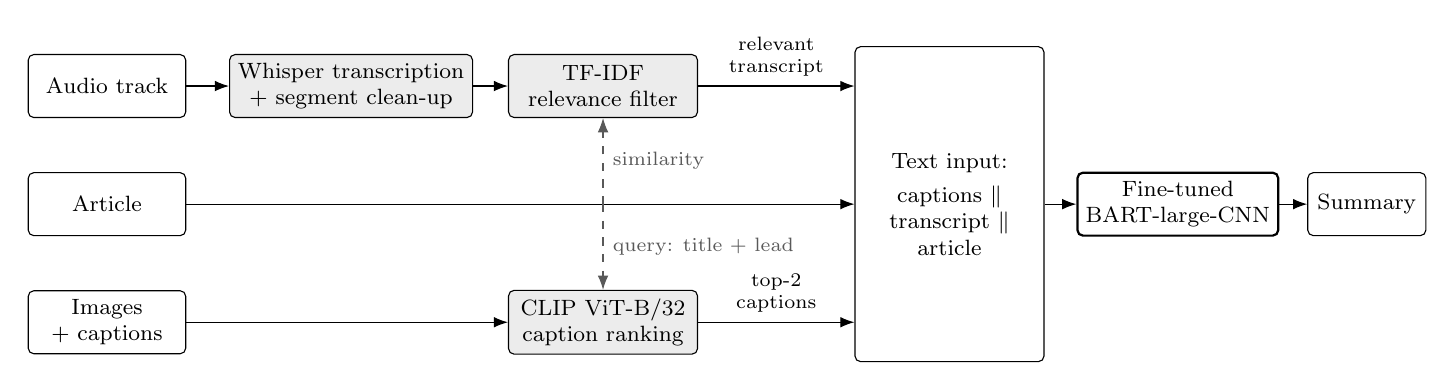
\begin{tikzpicture}[font=\footnotesize,
  box/.style={draw, rounded corners=2pt, align=center, minimum height=8mm, inner sep=3pt},
  sel/.style={box, fill=gray!15}, arr/.style={-{Latex[length=1.8mm]}},
  ctx/.style={arr, dashed, gray!70!black}, lab/.style={font=\scriptsize, align=center}]
% row 1: speech
\node[box, minimum width=20mm] (aud) at (10mm,0) {Audio track};
\node[sel, minimum width=27mm] (wh) at (41mm,0) {Whisper transcription\\+ segment clean-up};
\node[sel, minimum width=24mm] (rel) at (73mm,0) {TF-IDF\\relevance filter};
% row 2: article
\node[box, minimum width=20mm] (art) at (10mm,-15mm) {Article};
% row 3: images
\node[box, minimum width=20mm] (img) at (10mm,-30mm) {Images\\+ captions};
\node[sel, minimum width=24mm] (clip) at (73mm,-30mm) {CLIP ViT-B/32\\caption ranking};
% merge and summarize
\node[box, minimum width=24mm, minimum height=40mm] (inp) at (117mm,-15mm)
  {Text input:\\[1mm] captions $\|$\\ transcript $\|$\\ article};
\node[box, line width=0.8pt, minimum width=22mm] (bart) at (146mm,-15mm) {Fine-tuned\\BART-large-CNN};
\node[box, minimum width=15mm] (sum) at (170mm,-15mm) {Summary};
% main flow
\draw[arr] (aud) -- (wh);
\draw[arr] (wh) -- (rel);
\draw[arr] (rel.east) -- node[lab, above] {relevant\\transcript} (rel.east -| inp.west);
\draw[arr] (art.east) -- (art.east -| inp.west);
\draw[arr] (img) -- (clip);
\draw[arr] (clip.east) -- node[lab, above] {top-2\\captions} (clip.east -| inp.west);
\draw[arr] (inp) -- (bart);
\draw[arr] (bart) -- (sum);
% article used as the reference for both filters
\draw[ctx] (rel.south |- art.east) -- node[lab, right] {similarity} (rel.south);
\draw[ctx] (clip.north |- art.east) -- node[lab, right] {query: title + lead} (clip.north);
\end{tikzpicture}
\caption{Proposed pipeline. Speech and images are converted to text and filtered, then placed before the article as one text input to BART. Grey boxes are frozen or non-trained components; dashed arrows show the article acting as the reference for both filters.}
\label{fig:pipeline}
\end{figure*}

\begin{table}[t]
\caption{Unique stories per split (one copy per duplicate group). Captions, speech and relevant speech are subsets of the Daily Mail stories.}
\label{tab:data}
\centering
\begin{tabular}{lrrr}
\toprule
 & Train & Val & Test \\
\midrule
Stories               & 1{,}358 & 159 & 418 \\
\quad CNN             & 171 & 25 & 49 \\
\quad Daily Mail      & 1{,}187 & 134 & 369 \\
With image captions   & 1{,}086 & 122 & 338 \\
With speech           & 908 & 106 & 294 \\
With relevant speech  & 453 & 52 & 151 \\
\bottomrule
\end{tabular}
\end{table}

\subsection{Data preparation}
MM-AVS~\cite{fu2021mmavs} stores each story as a folder. A Daily Mail folder holds the article, reference highlights, a title, up to four images with captions, a video and its audio track; CNN stories have no images or audio. After removing incomplete folders we obtained 2{,}224 article--summary pairs and 1{,}935 unique stories (Table~\ref{tab:data}).

We found and repaired three data problems. First, some stories were scraped up to 12 times, giving 892 near-duplicate pairs. We grouped copies by union-find over exact matches and 8-word-shingle Jaccard similarity above 0.3, so that no story crosses a split, and kept one copy per group for training and evaluation. Second, about 70\% of Daily Mail highlight files had sentences joined with no separator (``last FridayRaiders seen''); we re-split them using a whitelist of genuine camel-case words collected from the articles. Third, we separated joined article sentences and removed datelines and boilerplate.

\subsection{Text summarizer}
The summarizer is BART-large-CNN~\cite{lewis2020bart}, fine-tuned on the training split. Extra modalities enter only as text placed before the article, in the form ``Image captions: \ldots{} $\|$ Video transcript: \ldots{} $\|$ Article: \ldots''. The model, loss and decoding are therefore the same in every experiment. Placing the extra text first means that truncation at 1{,}024 tokens can only remove the end of the article. CNN inputs are identical in all variants.

\subsection{Image stage: CLIP caption selection}
We use a frozen CLIP ViT-B/32 model~\cite{radford2021clip}. Because CLIP reads at most 77 tokens, the article is represented by its title and first two sentences. Each image $I_i$ is scored against this query $q$ by cosine similarity between the CLIP image and text embeddings $f_I$ and $f_T$:
\begin{equation}
s_i = \frac{f_I(I_i)\cdot f_T(q)}{\lVert f_I(I_i)\rVert\,\lVert f_T(q)\rVert}.
\label{eq:clip}
\end{equation}
Each caption inherits the score of its image.

Captions follow image order when the counts match, which holds for 71\% of stories. Otherwise we take the one-to-one assignment with the highest total image--caption similarity. In all, 90\% of captions are aligned to an image, and the remainder are ranked by their own text similarity to the query. The \texttt{clip\_top2} variant uses the two highest-ranked captions. Its controls are \texttt{all\_captions} and \texttt{random2}, which uses two captions chosen at random with a fixed per-story seed.

The same scores can also select a cover image directly, by taking the image most similar to the generated summary or to the article lead.

\subsection{Audio stage: Whisper transcripts with relevance filter}
We transcribe the first 90\,s of each clip with Whisper large-v3-turbo~\cite{radford2023whisper}, since BART has room for only about 100 transcript words beside the article. Segments with a no-speech probability of at least 0.6 or an average log-probability of $-1.0$ or lower are dropped, because such segments are likely to be non-speech or unreliable. Transcripts with fewer than 5 remaining words are discarded, and at most the first 100 words are kept.

Relevance $r(t,a)$ is the cosine similarity between the TF-IDF vectors of transcript $t$ and article $a$. Using a random permutation $\pi$ of the training stories, the threshold is the 99th percentile of similarities over mismatched pairs:
\begin{equation}
\tau = P_{99}\left(\{\, r(t_i, a_{\pi(i)}) : \pi(i)\neq i \,\}\right),
\label{eq:tau}
\end{equation}
which gives $\tau=0.10$ over 907 training pairs. A transcript is kept only if $r(t,a)>\tau$, so it must resemble its article more than 99\% of random pairings do. The vocabulary and threshold use training data only, and all settings were fixed before any transcript-variant result was seen. We compare all transcripts, relevant transcripts only, and \texttt{clip\_top2} combined with relevant transcripts.

% ===========================================================================
\section{Experimental Setup}
\textit{Hardware.} Training used a Kaggle Tesla T4 GPU with mixed precision and gradient checkpointing, peaking at 8.2\,GB of memory and taking about 25 minutes per variant. CLIP scoring of 4{,}789 images took 3.1 minutes, and transcription ran on an 8\,GB Apple M1 laptop.

\textit{Training and decoding.} We used AdamW with a learning rate of $2\times10^{-5}$, weight decay of 0.01, 10\% linear warm-up and an effective batch size of 8. Source and target limits were 1{,}024 and 192 tokens, with seed 42. The best epoch was chosen by mean validation ROUGE-1/2/L, from 6 epochs for the text baseline and 4 for the multimodal runs. Decoding, fixed before testing, used beam size 4, no repeated trigrams, length penalty 2.0 and 20--160 new tokens.

\textit{Evaluation.} We report ROUGE-1, ROUGE-2, ROUGE-L and ROUGE-Lsum F1 (abbreviated R-1, R-2, R-L and R-Lsum) with stemming, and compare variants with a paired bootstrap. With $d_k$ the score difference between a variant and its baseline on story $k$ of $n$, and $\bar{d}^{(b)}$ the mean of $d$ over resample $b$ of the $n$ stories,
\begin{equation}
p = \frac{1}{B}\sum_{b=1}^{B}\mathbb{1}\left[\bar{d}^{(b)}>0\right], \quad B=10{,}000.
\label{eq:boot}
\end{equation} Two identical text-only runs differed by up to 0.6 points, so we count a gain only if it exceeds 0.6 points and the bootstrap gives $p\ge0.95$.

\textit{Human study.} We sampled 100 Daily Mail test stories with at least two images. Annotators saw the title, the generated summary and the images in shuffled order, and chose the best cover image or ``none''. We collected 120 labels from three people, one of whom completed two of the four label files. Twenty stories were labelled twice, 15 of them by two different people.

% ===========================================================================
\section{Results and Analysis}
\label{sec:results}

\begin{table}[t]
\caption{Test ROUGE F1 (\%), 418 stories. Pretrained vs.\ fine-tuned BART-large-CNN on article text only.}
\label{tab:text}
\centering
\begin{tabular}{lcccc}
\toprule
Model & R-1 & R-2 & R-L & R-Lsum \\
\midrule
Pretrained (zero-shot) & 39.99 & 17.12 & 26.78 & 35.51 \\
Fine-tuned             & \textbf{42.48} & \textbf{18.78} & \textbf{28.75} & \textbf{37.73} \\
\bottomrule
\end{tabular}
\end{table}

\begin{table}[t]
\caption{Summary properties on the test set. $^{*}$Human highlights often add background knowledge not stated in the article.}
\label{tab:behaviour}
\centering
\begin{tabular}{lccc}
\toprule
Property & Human & Pretrained & Fine-tuned \\
\midrule
Words per summary                & 59 & 61 & 69 \\
Sentences copied from article    & 2\% & 47\% & 26\% \\
Name/number absent from article  & 49\%$^{*}$ & 3\% & 13\% \\
Ends mid-sentence                & -- & 1.4\% & 5.7\% \\
\bottomrule
\end{tabular}
\end{table}

\begin{table}[t]
\caption{Test ROUGE F1 (\%) by input, 418 stories. Same training and decoding for every row. Each block is one run with its own article-only baseline; $\Delta$ = R-2 gain over that baseline; $p$ = paired bootstrap probability of beating it (R-2).}
\label{tab:mm}
\centering
\setlength{\tabcolsep}{3pt}
\resizebox{\columnwidth}{!}{%
\begin{tabular}{lccccrc}
\toprule
Input & R-1 & R-2 & R-L & R-Lsum & $\Delta$ & $p$ \\
\midrule
Article only (run 4) & 42.62 & 18.85 & 28.69 & 37.93 & --    & --    \\
+ all captions      & \textbf{44.07} & \textbf{20.98} & \textbf{29.95} & \textbf{39.32} & +2.12 & 1.00 \\
+ CLIP top-2        & 43.67 & 20.05 & 29.49 & 38.88 & +1.19 & 0.99 \\
+ random-2          & 43.18 & 19.31 & 29.01 & 38.35 & +0.45 & 0.85 \\
\midrule
Article only (run 5)   & 42.28 & 18.58 & 28.57 & 37.42 & --    & --   \\
+ transcript, all      & 42.09 & 18.33 & 27.90 & 37.39 & $-$0.25 & 0.23 \\
+ transcript, relevant & 42.76 & 18.87 & 28.88 & 38.10 & +0.29 & 0.80 \\
+ CLIP-2 + relevant tr.& \textbf{43.37} & \textbf{19.92} & \textbf{29.14} & \textbf{38.80} & +1.34 & 1.00 \\
\bottomrule
\end{tabular}}
\end{table}

\begin{table}[t]
\caption{Test ROUGE F1 (\%) on the 369 Daily Mail stories only. CNN inputs never change, so this view shows the effect on stories that can receive extra modalities.}
\label{tab:dm}
\centering
\begin{tabular}{lcccc}
\toprule
Input & R-1 & R-2 & R-L & R-Lsum \\
\midrule
Article only (run 4) & 43.56 & 19.27 & 29.05 & 38.71 \\
+ all captions       & \textbf{45.30} & \textbf{21.65} & \textbf{30.56} & \textbf{40.32} \\
+ CLIP top-2         & 44.80 & 20.78 & 30.18 & 39.87 \\
+ random-2           & 44.26 & 19.88 & 29.40 & 39.25 \\
\midrule
Article only (run 5)   & 42.80 & 18.72 & 28.82 & 37.77 \\
+ transcript, all      & 42.95 & 18.75 & 28.13 & 38.09 \\
+ transcript, relevant & 43.80 & 19.40 & 29.24 & 38.91 \\
+ CLIP-2 + relevant tr.& \textbf{44.42} & \textbf{20.55} & \textbf{29.69} & \textbf{39.65} \\
\bottomrule
\end{tabular}
\end{table}

\begin{figure}[t]
\centering
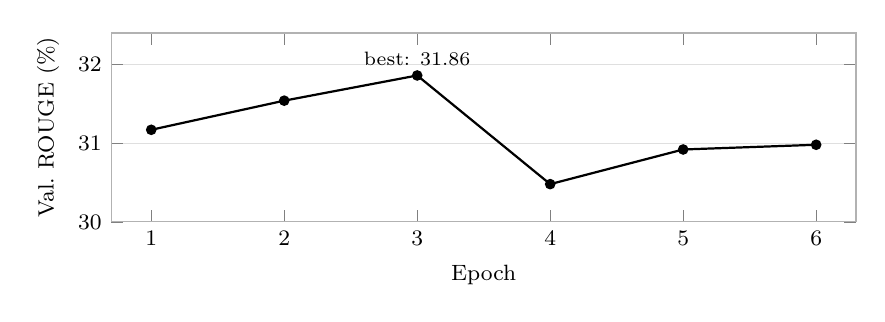
\begin{tikzpicture}
\begin{axis}[scale only axis, width=0.78\columnwidth, height=24mm, font=\footnotesize,
  xmin=0.7, xmax=6.3, ymin=30, ymax=32.4, xtick={1,2,3,4,5,6}, ytick={30,31,32},
  xlabel={Epoch}, ylabel={Val.\ ROUGE (\%)},
  ymajorgrids, grid style={gray!25}, axis line style={gray!60}]
\addplot[black, line width=0.8pt, mark=*, mark size=1.5pt] coordinates
  {(1,31.17) (2,31.54) (3,31.86) (4,30.48) (5,30.92) (6,30.98)};
\node[font=\scriptsize, above] at (axis cs:3,31.86) {best: 31.86};
\end{axis}
\end{tikzpicture}
\caption{Text baseline: mean validation R-1/2/L per epoch. Epoch 3 is selected for testing.}
\label{fig:epochs}
\end{figure}

\begin{figure}[t]
\centering
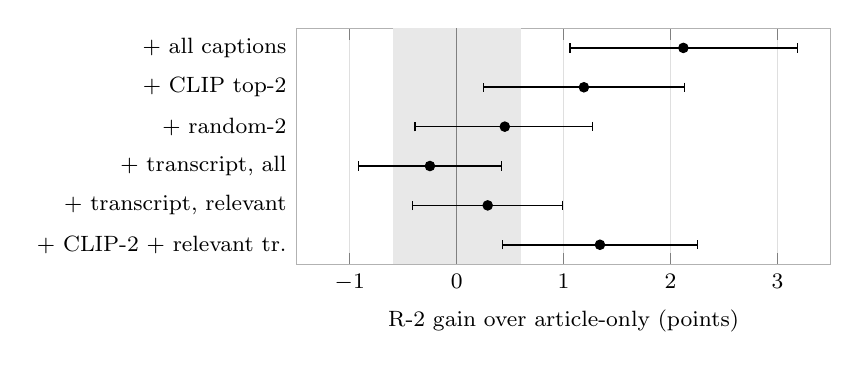
\begin{tikzpicture}
\begin{axis}[scale only axis, width=0.56\columnwidth, height=30mm, font=\footnotesize,
  xmin=-1.5, xmax=3.5, ymin=0.5, ymax=6.5, y dir=reverse,
  ytick={1,2,3,4,5,6},
  yticklabels={+ all captions, + CLIP top-2, + random-2, {+ transcript, all}, {+ transcript, relevant}, + CLIP-2 + relevant tr.},
  xlabel={R-2 gain over article-only (points)},
  xmajorgrids, grid style={gray!25}, ytick style={draw=none}, axis line style={gray!60}]
\fill[gray!18] (axis cs:-0.6,0.5) rectangle (axis cs:0.6,6.5);
\draw[gray] (axis cs:0,0.5) -- (axis cs:0,6.5);
\addplot[only marks, mark=*, mark size=1.7pt, black,
  error bars/.cd, x dir=both, x explicit, error bar style={black, line width=0.6pt}]
  coordinates {
  (2.12,1) += (1.07,0) -= (1.06,0)
  (1.19,2) += (0.94,0) -= (0.94,0)
  (0.45,3) += (0.82,0) -= (0.84,0)
  (-0.25,4) += (0.67,0) -= (0.67,0)
  (0.29,5) += (0.70,0) -= (0.70,0)
  (1.34,6) += (0.91,0) -= (0.91,0)};
\end{axis}
\end{tikzpicture}
\caption{R-2 gain over each run's article-only baseline, all 418 test stories, with 95\% paired bootstrap intervals. The shaded band is run-to-run noise ($\pm$0.6 points).}
\label{fig:gains}
\end{figure}

\begin{table}[t]
\caption{Where the caption gain comes from (Daily Mail test). R-2 gain over article-only, split by whether a reference sentence nearly copies a caption ($\ge$70\% bigram overlap).}
\label{tab:overlap}
\centering
\begin{tabular}{lcc}
\toprule
 & Copy stories & Other stories \\
 & ($n=49$) & ($n=289$) \\
\midrule
+ all captions & +9.79 & +1.11 \\
+ CLIP top-2   & +6.37 & +0.86 \\
+ random-2     & +1.97 & +0.37 \\
\bottomrule
\end{tabular}
\end{table}

\begin{table}[t]
\caption{Cover-image selection vs.\ human choice (precision@1, 112 labels on 100 Daily Mail test stories; 95\% bootstrap CI).}
\label{tab:cover}
\centering
\begin{tabular}{lc}
\toprule
Method & P@1 (\%) \\
\midrule
CLIP: image vs.\ fine-tuned summary & 40.2 [31.3, 49.1] \\
CLIP: image vs.\ article lead        & 42.9 [33.9, 51.8] \\
Lead (first) image                  & 27.7 [19.6, 36.6] \\
Random image                        & 30.3 \\
\bottomrule
\end{tabular}
\end{table}

\begin{table}[t]
\caption{Effect of speech transcripts by story group (gain over run-5 article-only, ROUGE points; $^{*}$ = paired bootstrap $p\ge0.95$ in that direction).}
\label{tab:audio}
\centering
\setlength{\tabcolsep}{4pt}
\begin{tabular}{lcccc}
\toprule
 & \multicolumn{2}{c}{Relevant ($n{=}151$)} & \multicolumn{2}{c}{Irrelevant ($n{=}143$)} \\
 & R-1 & R-L & R-1 & R-L \\
\midrule
+ transcript, all      & +0.80 & $-$0.57 & $-$0.20 & $-$1.01$^{*}$ \\
+ transcript, relevant & +1.98$^{*}$ & +0.95 & (not added) & (not added) \\
\bottomrule
\end{tabular}
\end{table}

\subsection{Text baseline}
Fine-tuning improves R-1 by 2.5, R-2 by 1.7 and R-L by 2.0 points (Table~\ref{tab:text}), with $p\ge0.999$ on all metrics. The 95\% interval for fine-tuned R-1 is [41.29, 43.54], against [38.71, 41.10] for the pretrained model. Fig.~\ref{fig:epochs} shows validation performance peaking at epoch 3 of 6. Training loss keeps falling from 1.81 to 0.63 while validation loss rises from 1.72 to 2.16, a clear sign of over-fitting.

Table~\ref{tab:behaviour} shows how the outputs change. The fine-tuned model copies far fewer sentences from the article (26\% against 47\%), but stories containing a name or number absent from the article rise from 3\% to 13\%. This is the faithfulness risk described in~\cite{maynez2020faithfulness}, and ROUGE does not penalize it.

Data cleaning proved essential. Before the glued highlights were repaired, fine-tuning appeared to lower R-Lsum from 30.6 to 27.7, because the model had learned to produce glued words.

\subsection{Image captions}
All caption variants score above article-only (Table~\ref{tab:mm}, Fig.~\ref{fig:gains}). All captions and CLIP top-2 pass the noise rule on R-2, while random-2 does not. The effect is larger on the Daily Mail stories that can actually receive captions (Table~\ref{tab:dm}), where all captions gain 1.74 R-1 and 2.38 R-2 points.

To isolate CLIP's selection, we compare on the 216 Daily Mail test stories where CLIP and random selection differ. There, CLIP top-2 beats random-2 by 1.74 R-1, 1.86 R-2 and 1.91 R-L points ($p\ge0.999$), and random-2 does not beat article-only. Over all stories the gap is only 0.5--0.9 points and is not significant. This subset was examined after the run, although it is defined only by the inputs and not by any score.

An important caveat appears in Table~\ref{tab:overlap}. In 49 of 338 Daily Mail test stories with captions (14.5\%), a reference sentence nearly duplicates a caption, which suggests that editors reuse caption text in highlights. The model learns this behaviour: 38\% of its sentences match a caption when it sees all captions, against 8\% for the article-only model. Most of the gain lies in those 49 stories. Elsewhere it falls to 0.86--1.11 R-2 points ($p=0.96$--$0.98$). Only 5\% of reference content words occur in captions but not in the article, so we suspect captions act mainly as a signal of what the editor considered important rather than as a source of new facts.

Table~\ref{tab:cover} gives the cover-image results. CLIP scored against the fine-tuned summary matches the human choice 40.2\% of the time, ahead of the first image at 27.7\% ($p=0.99$); its interval only narrowly excludes the expected random rate of 30.3\%. Scoring against the article lead performs similarly. Annotators chose ``none'' for 8 of 120 labels and agreed on 80\% of the 15 doubly labelled stories (chance 23\%, $\kappa\approx0.74$), although this sample is small. People did not favour the first image, even though it is CLIP's top choice in 44\% of stories.

\subsection{Speech transcripts}
Of 1{,}690 Daily Mail stories, 1{,}673 have audio, one file of which could not be read; Table~\ref{tab:data} gives the speech and relevant counts. The true article is the best TF-IDF match for 42\% of Whisper transcripts on the test stories examined, against 27\% for the dataset's own transcripts. Many clips are generic, such as an investment advertisement attached to a story about immigration.

Unfiltered speech does not help (Table~\ref{tab:mm}). Adding all transcripts changes R-1 by $-0.19$ and R-L by $-0.68$, a significant loss on R-L. On the 143 stories with an irrelevant transcript, the R-L loss reaches 1.01 points (Table~\ref{tab:audio}). Relevant transcripts do help where they are used: on the 151 test stories that receive one, the gain is 1.98 R-1, 1.69 R-2 and 1.92 R-Lsum points ($p\ge0.999$). As a check on run noise, the same variant scores 0.47 R-1 points higher on the 143 stories whose input it leaves unchanged, so the true effect is probably somewhat smaller. Over all 418 stories the gain is diluted to 0.29--0.68 points, and only R-Lsum (0.68, $p=0.96$) passes the noise rule. The filter itself matters: relevant transcripts beat all transcripts by 0.67 R-1 and 0.99 R-L points ($p=0.97$ and $0.998$).

Only about 1\% of summary content words come solely from the transcript, so speech appears to serve as context rather than as copied text, and the caption caveat does not apply in the same way.

Combining CLIP top-2 with relevant transcripts beats article-only by 1.09 R-1, 1.34 R-2 and 1.38 R-Lsum points ($p\ge0.99$). However, it is not better than CLIP top-2 alone from the earlier run ($-0.30$ R-1, not significant), and this comparison crosses two runs whose article-only baselines differ by 0.34 points. Captions therefore carry most of the multimodal gain, and we find no measurable benefit from adding speech on top of them.

\subsection{Discussion}
The caption copying effect is easy to see in individual stories. In one Daily Mail story, the first reference sentence, ``Jon Benton said senior official from Foreign Office told him to stop investigation'', appears almost word for word in a caption. The all-captions model reproduces it while the article-only model paraphrases it, and R-2 rises by 0.58 on that story. Copying also grows with the amount of caption text shown: 15.3\% of sentences match a caption with random-2, 23.3\% with CLIP top-2 and 38.1\% with all captions. A high ROUGE gain therefore need not mean that the model has learned anything about the images themselves.

Selection still matters after allowing for this. CLIP top-2 and random-2 receive the same number of captions, yet only CLIP top-2 passes the noise rule, and the difference is clear where their selections differ. One plausible reason is that images closest to the article lead tend to show its main event, so their captions restate what the highlights also cover. We did not test this explanation directly.

Speech behaves differently. Whisper output is often conversational and off-topic, and a transcript placed before the article takes the first position in the input. We suspect this is why irrelevant transcripts lower R-L, which rewards correctly ordered content, but the design cannot confirm the cause. The filter is simple and costs almost nothing, yet it turned a loss into a gain. Its main weakness is that it is lexical, so a relevant clip phrased in different words is rejected.

Epoch selection also deserves caution. The caption-bearing \texttt{all\_captions}, \texttt{clip\_top2} and combined variants peaked at epoch 1, while the article-only baseline peaked at epoch 3 in one run and epoch 2 in another. With only 159 validation stories, validation differences of a few tenths of a point may be noise, so the selected epoch is itself uncertain.

Finally, the cost is low. Each variant trained in about 25 minutes on a free GPU, CLIP scoring took about 3 minutes, and transcribing all clips took several hours on a laptop with no paid compute. This makes the approach practical for small teams.

% ===========================================================================
\section{Conclusion and Future Work}
Converting images and speech to text and filtering them for relevance improves news summarization at small compute cost. Captions chosen with CLIP gave a significant gain while randomly chosen captions did not, and CLIP selected cover images that people preferred over the first image. Speech helped only after filtering, and unfiltered transcripts lowered R-L. Captions carried most of the combined gain.

These results have limits. Part of the caption gain reflects reuse of caption text in reference highlights, so we recommend that work on MM-AVS report results with and without such stories. We relied on ROUGE without human rating of summary quality, images and audio exist only for Daily Mail, each variant used one seed, the relevance filter is lexical, the cover-image study had three annotators, and only 49 CNN stories were available for testing.

Future work will add human evaluation of summaries, video frames, factual-consistency measures~\cite{kryscinski2020factcc}, generated captions~\cite{li2022blip} for images without captions, and a semantic relevance filter.

% ===========================================================================
\bibliographystyle{IEEEtran}
\bibliography{references}

\end{document}
